\documentclass[border=3.14mm]{standalone}

\usepackage{tikz}
\usepackage{ifthen}
\usetikzlibrary{math}
\begin{document}
\pagestyle{empty}

\pgfdeclarelayer{background}
\pgfsetlayers{background,main}

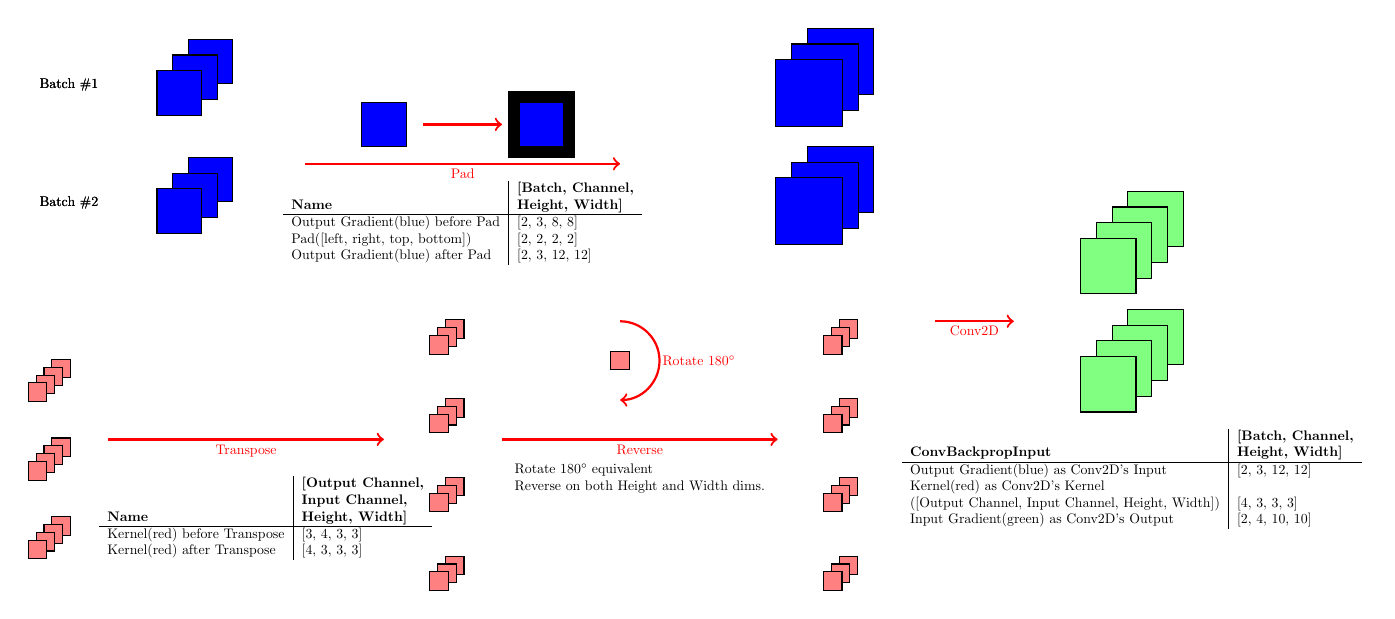
\begin{tikzpicture}[draw=black!50]
\tikzstyle{neuron}=[rectangle, draw=black, fill=black!25]
\tikzstyle{input neuron}=[neuron, fill=green!50, minimum size=20pt];
\tikzstyle{output neuron}=[neuron, fill=blue, minimum size=16pt];
\tikzstyle{pad output neuron}=[neuron, fill=black, minimum size=24pt];
\tikzstyle{output pad neuron}=[neuron, fill=blue, minimum size=24pt];
\tikzstyle{kernel neuron}=[neuron, fill=red!50, minimum size=6pt];
\tikzstyle{kline} = [red, thick]

% Draw the input layer nodes
\tikzmath{
    \batchsize = 2;
    \inputsize = 4;
    \outputsize = 3;
}

\foreach \bn in {1,...,\batchsize}
    \foreach \x in {1,...,\outputsize} {
        \tikzmath{
            real \bshift;
            \bshift = -3 * \bn - 1;
        }
        \node[scale=0.5, yshift = \bshift cm] () {Batch \#\bn};
        \node[output neuron, xshift=2cm, yshift = \bn * -1.5cm] () at (-\x * 0.2, -\x * 0.2) {};
    };

\foreach \x in {1,...,\outputsize}
    \foreach \y in {1,...,\inputsize} {
        \tikzmath{
            real \bshifta;
            \bshifta = -1 * \x - 4.5;
        }
        \node[kernel neuron, xshift=0cm, yshift=\bshifta cm] () at (-\y * 0.1, -\y * 0.1) {};
    };

\draw [->, kline] (0.5, -6.5) -- node[scale=0.5, anchor=north] {Transpose} (4, -6.5);

\node [scale=0.5, xshift=5cm, yshift=-15cm]() {
    \begin{tabular}{l|l} 
     & \textbf{[Output Channel,} \\
     & \textbf{Input Channel,} \\
    \textbf{Name} & \textbf{Height, Width]} \\
    \hline
    Kernel(red) before Transpose & [3, 4, 3, 3] \\
    Kernel(red) after Transpose & [4, 3, 3, 3] \\
    \end{tabular}
};

\foreach \x in {1,...,\inputsize}
    \foreach \y in {1,...,\outputsize} {
        \tikzmath{
            real \bshifta;
            \bshifta = -1 * \x - 4;
        }
        \node[kernel neuron, xshift=5cm, yshift=\bshifta cm] () at (-\y * 0.1, -\y * 0.1) {};
    };

\draw [->, kline] (3, -3) -- node[scale=0.5, anchor=north] {Pad} (7, -3);

\node[output neuron, xshift=4cm, yshift=-2.5 cm] () at (0, 0) {};

\node [scale=0.5, xshift=10cm, yshift=-7.5cm]() {
    \begin{tabular}{l|l} 
     & \textbf{[Batch, Channel,} \\
    \textbf{Name} & \textbf{Height, Width]} \\
    \hline
    Output Gradient(blue) before Pad & [2, 3, 8, 8] \\
    Pad([left, right, top, bottom]) & [2, 2, 2, 2] \\
    Output Gradient(blue) after Pad & [2, 3, 12, 12] \\
    \end{tabular}
};

\draw [->, kline] (4.5, -2.5) -- node[scale=0.5, anchor=north] {} (5.5, -2.5);

\node[pad output neuron, xshift=6cm, yshift=-2.5 cm] () at (0, 0) {};
\node[output neuron, xshift=6cm, yshift=-2.5 cm] () at (0, 0) {};

\node[kernel neuron, xshift=7cm, yshift=-5.5 cm] (A) at (0, 0) {};

\draw [->, kline] (7, -5) arc [start angle=90, end angle=-90, radius=0.5cm];

\node[kline, scale=0.5, xshift=16cm, yshift=-11 cm] (A) at (0, 0) {Rotate $180^{\circ}$};

\draw [->, kline] (5.5, -6.5) -- node[scale=0.5, anchor=north] {Reverse} (9, -6.5);

\node [scale=0.5, xshift=14.5cm, yshift=-14cm]() {
    \begin{tabular}{l} 
    Rotate $180^{\circ}$ equivalent \\
    Reverse on both Height and Width dims. \\
    \end{tabular}

};

\foreach \bn in {1,...,\batchsize}
    \foreach \x in {1,...,\outputsize} {
        \tikzmath{
            real \bshift;
            \bshift = -1.5 * \bn;
        }
        \node[output pad neuron, xshift=10cm, yshift = \bshift cm] () at (-\x * 0.2, -\x * 0.2) {};
    };

\foreach \x in {1,...,\inputsize}
    \foreach \y in {1,...,\outputsize} {
        \tikzmath{
            real \bshifta;
            \bshifta = -1 * \x - 4;
        }
        \node[kernel neuron, xshift=10cm, yshift=\bshifta cm] () at (-\y * 0.1, -\y * 0.1) {};
    };

\draw [->, kline] (11, -5) -- node[scale=0.5, anchor=north] {Conv2D} (12, -5);

\node [scale=0.5, xshift=27cm, yshift=-14cm]() {
    \begin{tabular}{l|l} 
     & \textbf{[Batch, Channel,} \\
    \textbf{ConvBackpropInput} & \textbf{Height, Width]} \\
    \hline
    Output Gradient(blue) as Conv2D's Input & [2, 3, 12, 12] \\
    Kernel(red) as Conv2D's Kernel & \\
    ([Output Channel, Input Channel, Height, Width]) & [4, 3, 3, 3] \\
    Input Gradient(green) as Conv2D's Output & [2, 4, 10, 10] \\
    \end{tabular}
};

\foreach \x in {1,...,\batchsize}
    \foreach \bn in {1,...,\inputsize} {
        \tikzmath{
            real \bshifta;
            \bshifta = -1.5 * \x - 2;
        }
        \node[input neuron, xshift=14cm, yshift = \bshifta cm] () at (-\bn * 0.2, -\bn * 0.2) {};
    };

\end{tikzpicture}
% End of code
\end{document}
